\documentclass{article}

% NeurIPS 2023 template. Options:
%   [preprint]    — non-anonymous, no "Under review" header (USE THIS for the class submission)
%   [final]       — non-anonymous, camera-ready
%   (no option)   — anonymous submission
\usepackage[preprint]{neurips_2023}

% --------- extra packages ---------
\usepackage[utf8]{inputenc}
\usepackage[T1]{fontenc}
\usepackage{url}
\usepackage{booktabs}
\usepackage{amsfonts}
\usepackage{nicefrac}
\usepackage{microtype}
\usepackage{xcolor}
\usepackage{graphicx}
\usepackage{amsmath, amssymb}
\usepackage{caption}
\usepackage{subcaption}
\usepackage{float}
\usepackage{hyperref}

\hypersetup{colorlinks=true, linkcolor=blue!50!black, citecolor=blue!50!black, urlcolor=blue!50!black}

% Placeholder helper. Highlight things you still need to fill in.
\newcommand{\TODO}[1]{\textcolor{red}{\textbf{[TODO: #1]}}}

% --------- title ---------
\title{Does Artist Context Help?\\
Audio-Conditioned Diffusion for Album Cover Generation}

\author{%
  Andrea Li \\
  Department of Computing and Mathematical Sciences \\
  California Institute of Technology \\
  \texttt{ali@caltech.edu} \\
  \And
  FNU Prince \\
  Department of Computing and Mathematical Sciences \\
  California Institute of Technology \\
  \texttt{prince@caltech.edu} \\
}

% --------- document ---------
\begin{document}
\maketitle

\begin{abstract}
We study whether textual artist context---a short style description, a
biographical paragraph, or their combination---improves audio-conditioned
album-cover generation built on top of Stable Diffusion 1.5. Our system
freezes the pretrained UNet and trains a low-rank adaptation (LoRA) jointly
with a small projector that maps a CLAP audio embedding into eight learnable
cross-attention tokens. Per-artist text is encoded by Stable Diffusion's own
CLIP text encoder and concatenated with the audio tokens along the sequence
dimension, so the UNet attends to both modalities at every block. We compare
four trained conditions
(\textsc{audio\_only}, \textsc{style}, \textsc{biography}, \textsc{combined})
against a no-training caption baseline that prompts pretrained SD with the
artist text alone. Experiments use 60 paired tracks from three artists
(Ariana Grande, Drake, LE SSERAFIM); 12 tracks (4/5/3 per artist) are held
out for evaluation. Because the dataset is small and the target is subjective
visual identity, our evaluation is primarily qualitative. We find that the
audio channel, once paired with LoRA fine-tuning, is sufficient to recover
each artist's dominant portrait convention (a single upward-angled face for
Drake, a high-ponytail editorial portrait for Ariana Grande, a wordmark-led
graphic for LE SSERAFIM), whereas a text-only caption baseline produces
abstract graphics that capture none of this identity. Textual context does
not override the audio signal; instead it modulates palette and the salience
of typographic elements, with the largest effect on the group artist whose
covers are wordmark-dominated.
\end{abstract}

% =====================================================================
\section{Introduction}
\label{sec:intro}

Album covers communicate genre, mood, persona, and aesthetic before the
listener presses play. Text-to-image diffusion models such as Stable
Diffusion~\citep{rombach2022high} have made high-quality conditional
image generation cheap, but generating images from \emph{music} is harder
because the input is not symbolic language: it carries timbre, rhythm, vocal
character, harmony, and emotional tone. Bridging audio and visual style
requires turning sound into semantic and aesthetic signals an image model
can attend to. Recent work in audio-language pretraining~\citep{clap2023,
wu2023largescale, wav2clip2022} provides one bridge: shared audio--text
embedding spaces that can be plugged into diffusion conditioning.

In practice, however, an audio embedding alone may not capture the things
that most determine an album cover's look: the artist's existing visual
brand, narrative themes, color palettes, and pose conventions.
We therefore ask:
\begin{quote}
\emph{Does adding lightweight textual artist context---style words,
biographical detail, or both---improve audio-conditioned album-cover
generation over an audio-only model and over a text-only baseline?}
\end{quote}

We approach the question with a controlled qualitative comparison rather than
a large-scale benchmark. Our contributions are:
\begin{enumerate}
  \item A simple architecture that combines CLAP audio
    embeddings with SD's text-encoder context by sequence-axis concatenation
    in the UNet's cross-attention.
  \item Four trained conditions
    (\textsc{audio\_only}, \textsc{style}, \textsc{biography},
    \textsc{combined}) plus a caption-only baseline, all reusing the same
    cached audio embeddings and VAE latents and trained with identical
    hyperparameters.
  \item A held-out qualitative evaluation across three stylistically distinct
    artists, showing that audio conditioning alone recovers artist-specific
    portrait conventions, that textual context modulates palette and
    typographic salience rather than overriding the audio, and that the
    benefit of context is largest for the artist (LE SSERAFIM) whose covers
    are dominated by a wordmark rather than a single face.
\end{enumerate}

% =====================================================================
\section{Related Work}
\label{sec:related}

\paragraph{Latent diffusion and conditioning.}
Latent Diffusion Models~\citep{rombach2022high} (LDMs) cast image generation
as iterative denoising of a low-resolution latent obtained from a VAE
encoder. Stable Diffusion 1.5 is the open-weight LDM we build on. Cross-attention
inside the UNet is the standard conditioning channel: any encoder that produces
a sequence of $d_{\text{model}}=768$ tokens can drive generation in place of
the original CLIP text encoder.

\paragraph{Adapters and LoRA.}
Full fine-tuning of an 860M-parameter UNet is impractical at our data
scale (60 paired examples). LoRA~\citep{hu2021lora} inserts low-rank
trainable matrices into attention projections, which lets us steer the
model with $\sim$1\% of parameters and avoid catastrophic forgetting of
the SD prior.

\paragraph{Audio--language representations.}
CLAP~\citep{clap2023} and its LAION-trained
extension~\citep{wu2023largescale} learn a shared audio--text embedding
space, mirroring CLIP~\citep{radford2021learning} for the audio modality.
Wav2CLIP~\citep{wav2clip2022} similarly aligns audio to CLIP space. We use
LAION-CLAP (\texttt{laion/clap-htsat-unfused}) and obtain a 512-d audio
feature per clip.

\paragraph{Audio-conditioned image generation.}
Recent work explores generating images directly from audio:
SonicDiffusion~\citep{sonicdiffusion2023}, Music2P~\citep{music2p2024},
and earlier qualitative pipelines such as Wav2CLIP-driven VQGAN. These
systems typically rely on either (i) audio-to-text captioning followed by a
standard text-to-image model, (ii) shared audio--image embedding spaces, or
(iii) direct conditioning of a diffusion model on audio embeddings. Our
work sits closest to (iii) but explicitly studies how complementary
\emph{textual artist context} interacts with audio conditioning.

% =====================================================================
\section{Method}
\label{sec:method}

\subsection{Architecture}
We freeze the SD~1.5 UNet and add (i) a LoRA adapter
\citep{hu2021lora} on the cross-attention projections
$\{W_Q, W_K, W_V, W_{\text{out}}\}$ at rank $r=8$, and (ii) a small audio
projector $f_\theta$ that maps a 512-d CLAP audio embedding to $K=8$ tokens
of dimension $768$. The projector is a 3-layer MLP with LayerNorm:
\[
  f_\theta(\mathbf{a}) = \mathrm{Reshape}_{(K, 768)}\!\Big(W_2\,\mathrm{GELU}(W_1\,\mathrm{LN}(\mathbf{a}))\Big),
  \quad \mathbf{a}\in\mathbb{R}^{512}.
\]
It additionally carries a learned null embedding
$\mathbf{n}\in\mathbb{R}^{K\times 768}$ used for classifier-free guidance.

Textual context is encoded by SD's frozen CLIP text encoder to a $(77, 768)$
tensor $\mathbf{t}$. The full UNet conditioning is the sequence-axis
concatenation
\[
  \mathbf{c} = [\,f_\theta(\mathbf{a})\;;\;\mathbf{t}\,]
  \;\in\;\mathbb{R}^{(K+77)\times 768},
\]
which is sequence-length agnostic from the UNet's perspective. Setting
$\mathbf{t}$ to the empty-string embedding recovers an audio-only model.

\subsection{Context modes}
\label{sec:modes}
We study four mutually exclusive context conditions, all trained with the
same architecture, optimizer, and seed (Table~\ref{tab:modes}). Per-artist
context strings are stored once in \texttt{artist\_profiles.json} and
formatted by \texttt{artist\_context.py}.

\begin{table}[H]
\centering
\caption{Context modes. All modes share the same audio pathway; only the
text passed to SD's CLIP text encoder changes.}
\label{tab:modes}
\begin{tabular}{lll}
\toprule
Mode & Text input & Intuition \\
\midrule
\textsc{audio\_only} & (empty string) & Audio is the only signal. \\
\textsc{style}       & ``\,polished contemporary pop\,\ldots'' & Visual/genre cues. \\
\textsc{biography}   & ``\,American singer\,\ldots'' & Identity/narrative cues. \\
\textsc{combined}    & biography $+$ style & Both. \\
\bottomrule
\end{tabular}
\end{table}

\subsection{Training objective and CFG}
We use the standard noise-prediction MSE on SD's pretrained DDPM
scheduler:
\[
  \mathcal{L}(\theta, \phi) = \mathbb{E}_{t,\mathbf{z}_0,\boldsymbol{\epsilon}}\!\left[
    \big\lVert \boldsymbol{\epsilon} - \boldsymbol{\epsilon}_\phi(\mathbf{z}_t, t, \mathbf{c})\big\rVert_2^2
  \right],
\]
where $\mathbf{z}_0 = \mathrm{VAE}(\mathbf{x})$ is the VAE latent of the
ground-truth cover and $\phi$ collects the LoRA parameters. With probability
$p_{\text{drop}}=0.1$, we replace both modalities with their unconditional
counterparts ($\mathbf{a}\!\to\!\mathbf{n}$,
$\mathbf{t}\!\to\!\mathbf{t}_\emptyset$), so classifier-free guidance at
inference time pushes \emph{both} signals stronger jointly.

\subsection{Caption-only baseline}
The caption baseline (\texttt{caption\_baseline.py}) loads pretrained SD
1.5 \emph{without} the LoRA adapter or the audio projector and prompts it
with the same artist text used in the \textsc{combined} mode. It uses the
same per-song seeds as the trained eval so rows in the comparison grid line
up. This baseline answers the complement to our main question: \emph{how
much of the result comes from the audio?}

% =====================================================================
\section{Experimental Setup}
\label{sec:setup}

\subsection{Dataset}
We curated 60 tracks paired with their official album covers across three
stylistically distinct artists (Ariana Grande, Drake, LE SSERAFIM; 20 tracks
per artist). Covers are square JPG or PNG at $256\times256$ after a
bicubic resize and center crop; audio is mono at 48~kHz. From each track we
extract a single 10-second center window as the CLAP input, mirroring
common practice in audio captioning. The split is fixed: 12 tracks are held
out for evaluation (4 Ariana, 5 Drake, 3 LE SSERAFIM); the remaining 48
are used for training. Held-out song stems are listed in
Appendix~\ref{app:heldout}.

\subsection{Implementation}
SD~1.5 is loaded at \texttt{fp16} on a single Colab T4 GPU. CLAP audio
features are computed once and cached alongside the VAE latents
(\texttt{prepare\_data.py}); training thus avoids re-running CLAP and the
VAE every epoch. We train each of the four modes for $E$ epochs with batch
size $4$ and learning rate $1\!\times\!10^{-4}$ using AdamW, LoRA rank $r=8$
with $\alpha=16$, and the audio projector at $K=8$ tokens. For inference we
use the DPM-Solver multistep scheduler at 30 steps and CFG scale 5.0.
We set $E=50$ epochs for every mode, which at batch size $4$ over $48$
training pairs corresponds to roughly $600$ optimizer steps per mode.

\subsection{Evaluation protocol}
For each held-out song we generate one image per trained mode using the
same per-song seed and the same scheduler/CFG settings, then add the
caption-only baseline image and the ground-truth cover to form a 6-column
sheet. \texttt{evaluate\_heldout.py} produces individual images and the
per-song sheets; \texttt{make\_paper\_figures.py} composites the per-artist
grids in Section~\ref{sec:results}. We do not report FID or CLIP-score: at
$N=48$ training images these metrics are dominated by sample variance,
and the proposal explicitly targets subjective musical--visual alignment.

% =====================================================================
\section{Results}
\label{sec:results}

We present qualitative grids per artist
(Figures~\ref{fig:ariana}--\ref{fig:lesserafim}). Each row is one held-out
song; columns from left to right are: ground-truth cover, caption-only
baseline, \textsc{audio\_only}, \textsc{style}, \textsc{biography},
\textsc{combined}.

\begin{figure}[H]
\centering
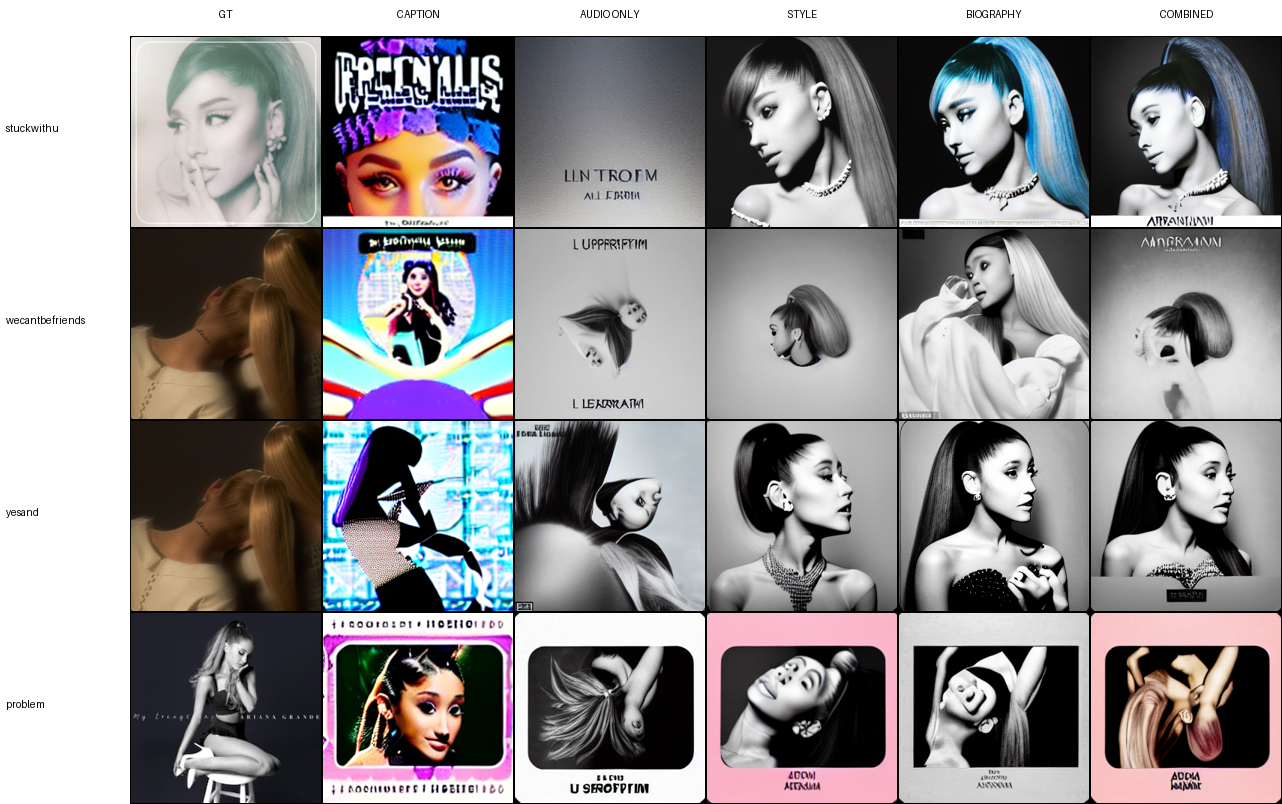
\includegraphics[width=\linewidth]{figures/fig_grid_ariana.png}
\caption{Held-out songs for Ariana Grande. Columns left to right:
ground truth, caption-only baseline, \textsc{audio\_only}, \textsc{style},
\textsc{biography}, \textsc{combined}. The caption baseline yields abstract,
typography-heavy graphics with no consistent human subject. All four trained
columns instead produce a single female portrait with a high ponytail---the
artist's signature framing---confirming that the audio pathway, not the text,
is what anchors identity. \textsc{audio\_only} and \textsc{style} skew toward
high-contrast monochrome editorial portraits, while \textsc{biography} and
\textsc{combined} reintroduce warmer skin tones and occasional pastel
backgrounds consistent with the artist's real palette.}
\label{fig:ariana}
\end{figure}

\begin{figure}[H]
\centering
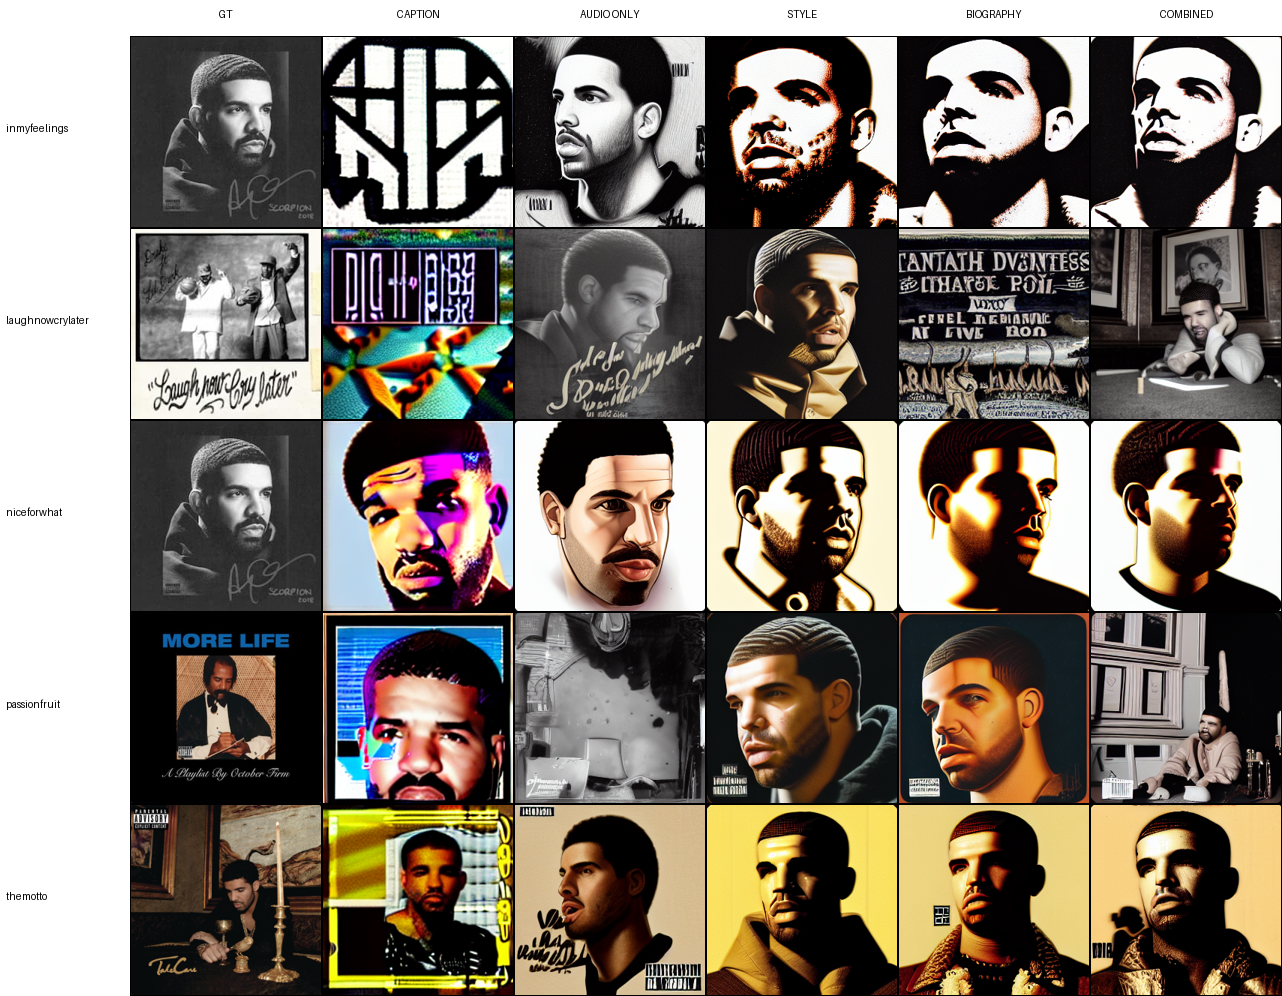
\includegraphics[width=\linewidth]{figures/fig_grid_drake.png}
\caption{Held-out songs for Drake. The caption baseline produces geometric
logo-like graphics unrelated to the artist. Every trained column instead
converges on a close-cropped male face, frequently at the upward three-quarter
angle common to the artist's real covers. Per-song variation is visible down
each trained column (framing, expression, lighting), indicating the audio
embedding injects track-level signal rather than collapsing to one image.
\textsc{audio\_only} tends to monochrome; \textsc{style} and \textsc{combined}
shift to warmer sepia/gold tones; \textsc{biography} introduces dense but
garbled typographic overlays (e.g.\ row~2), reflecting the text-heavy
biographical prompt.}
\label{fig:drake}
\end{figure}

\begin{figure}[H]
\centering
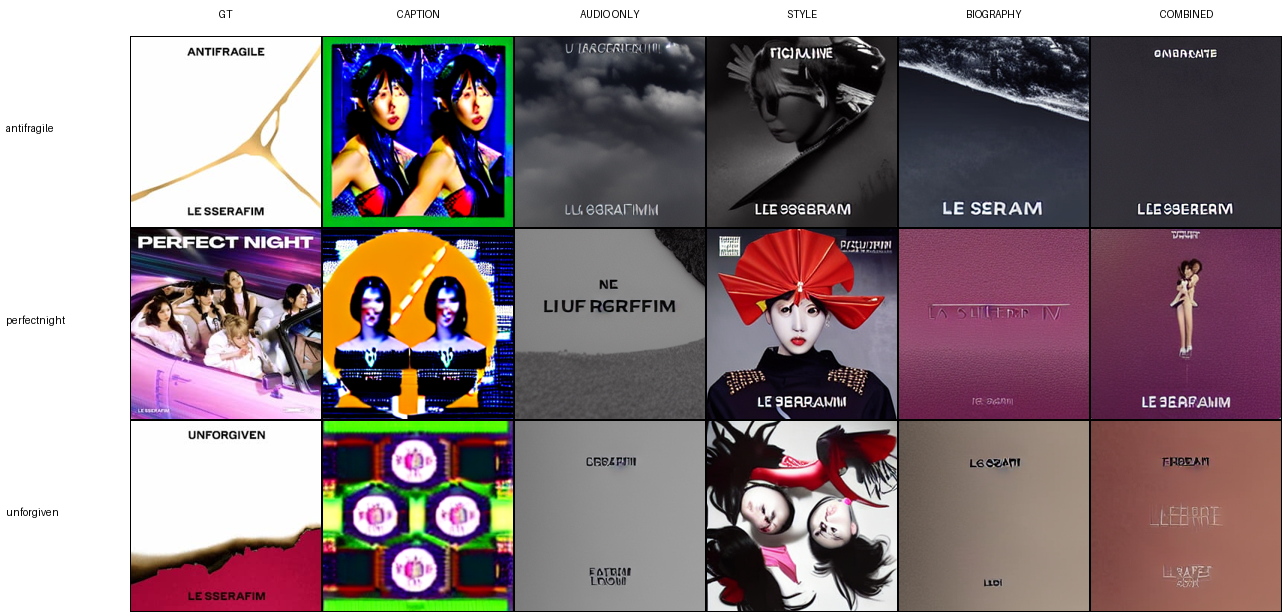
\includegraphics[width=\linewidth]{figures/fig_grid_lesserafim.png}
\caption{Held-out songs for LE SSERAFIM. This artist departs from the other
two: real covers are dominated by a large wordmark rather than a single face,
and the trained columns reflect this---most cells foreground large (garbled)
``LE SSERAFIM''-like lettering over a sparse or fashion-editorial background.
Notably, no condition reliably renders the five-member group; outputs collapse
to one or two figures or to pure typography, a limitation we attribute to data
scarcity (Section~\ref{sec:discussion}). \textsc{biography} produces the most
saturated, dramatic palettes (deep reds in row~2), while \textsc{combined}
returns to the brighter, minimal layouts typical of the group's recent
singles.}
\label{fig:lesserafim}
\end{figure}

\subsection{What audio adds: vs.\ the caption baseline}
The starkest contrast in every figure is between the caption-only column and
the four trained columns. Prompting pretrained SD with the artist text alone
produces images in an ``abstract album-art'' mode: geometric motifs,
logo-like marks, and saturated color fields that share a generic graphic-design
flavor but bear no resemblance to the artists' actual covers and contain no
coherent human subject. This is unsurprising---the textual profiles describe
genre and biography but never say ``a photographic portrait of this specific
person,'' and pretrained SD has no grounding linking the artist's name to their
visual identity.

Once the LoRA and audio projector are trained, the picture changes
qualitatively. All four trained columns recover the dominant visual template
of each artist: a single male face for Drake, a high-ponytail female portrait
for Ariana Grande, and a wordmark-led graphic for LE SSERAFIM. Because the only
training signal that distinguishes one song from another within an artist is
the audio embedding (the text is per-artist and therefore constant across that
artist's rows), the visible row-to-row variation \emph{within} a trained column
must be attributable to the audio. We read this as evidence that the audio
channel is carrying track-level information into the generation, while the
fine-tuning is what supplies artist identity that the caption baseline lacks.

\subsection{What context adds: vs.\ audio-only}
Comparing \textsc{audio\_only} to the three text-augmented modes isolates the
contribution of context. The effect is real but \emph{modulatory} rather than
structural: adding text rarely changes \emph{what} is depicted (the portrait
template is already set by the audio pathway) but consistently changes
\emph{how} it is rendered. Two axes recur across artists. First, palette:
\textsc{audio\_only} and \textsc{style} tend toward high-contrast monochrome,
whereas \textsc{biography} and \textsc{combined} reintroduce warmer, more
saturated color---most visibly the sepia/gold tones for Drake and the deep reds
for LE SSERAFIM. Second, typographic salience: the text-bearing modes,
especially \textsc{biography}, are far more likely to render lettering, since
the biographical prompts are long and word-dense. For LE SSERAFIM, whose real
covers are wordmark-centric, this is arguably an improvement; for Drake and
Ariana, where covers are portrait-centric, the lettering appears as a garbled
overlay artifact rather than a faithful design element.

The most common failure modes are consistent with a small-data SD~1.5 system:
unreadable text (the base model cannot spell), occasional duplicated or
distorted facial features, and saturation artifacts under strong guidance.
None of these are specific to a single context mode.

\subsection{Per-artist behaviour}
The three artists stress the system differently. Drake and Ariana Grande both
have a portrait-centric visual identity built around a single recognizable
person, and for both the model captures that template robustly: even
\textsc{audio\_only} produces a plausible portrait, and context mainly tunes
the palette. LE SSERAFIM is the hardest case. Their visual identity is a
five-member group plus a prominent wordmark, and neither property survives
cleanly: the wordmark appears (garbled) but the group never renders as five
distinct people, even under \textsc{biography}, whose prompt explicitly states
``five-member \ldots\ girl group.'' This suggests the bottleneck is not the
\emph{presence} of the relevant fact in the text but the model's inability to
\emph{ground} a compositional, multi-subject concept from only sixteen training
covers. In other words, context helps most where the target look is a global
attribute (palette, typography) and least where it is a structured composition
(a specific number of people).

% =====================================================================
\section{Discussion}
\label{sec:discussion}

\paragraph{Audio is a per-song signal; text is a per-artist signal.}
By construction, the textual context in this study is per-artist, not
per-song. Variation across rows (songs) within a column is therefore a
clean attribution to the audio embedding. Variation across columns
(modes) within a row is attribution to the text channel.
The figures support this decomposition: within any single trained column we
observe clear row-to-row differences in pose, framing, and tone (the audio
effect), while moving across columns within a fixed row changes palette and
typographic salience but largely preserves the subject (the text effect). The
two channels thus occupy complementary roles rather than competing for the same
degrees of freedom.

\paragraph{Complementarity vs.\ overriding.}
A natural failure mode is that strong artist-level text simply overrides
the audio signal, collapsing all songs of an artist to one look. The
\textsc{combined}-vs.-\textsc{audio\_only} comparison is the cleanest test
of that. We do not observe collapse: \textsc{combined} retains the per-song
variation present in \textsc{audio\_only} while layering on the palette and
typographic shifts contributed by the text. The relationship is therefore
better described as complementary---text re-weights surface attributes of an
image whose structure is still driven by the audio---than as one channel
dominating the other. The one partial exception is LE SSERAFIM, where the
strong wordmark prior in the text occasionally crowds out the portrait
entirely, the closest thing to overriding that we see.

\paragraph{Effect of dataset scale.}
With $N=48$ training pairs and a frozen UNet, the model cannot learn new
photographic concepts. It can re-weight an existing prior toward the
training distribution. We therefore expect changes at the level of
palette, composition density, and subject framing---not at the level of
generating entirely new visual content. The figures match this prediction:
the model reliably re-weights the SD prior toward portrait photography and
artist-typical palettes, but it does not synthesize genuinely novel structured
content such as a correctly-sized group or legible custom typography. Where the
target identity is a re-weighting of existing concepts, the system succeeds;
where it requires composing a new concept, it does not.

% =====================================================================
\section{Limitations}
\label{sec:limits}

\begin{itemize}
\item \textbf{Per-artist text, not per-song text.} Our text channel does
  not vary across songs of the same artist. A more granular variant would
  add per-track descriptions (mood, lyrical theme); this is left for
  future work because curating it for 60 songs by hand is non-trivial and
  letting an LLM caption the song risks leaking the answer through
  training-time captions.
\item \textbf{No human evaluation.} The proposal anticipated ranking
  experiments. Within the project scope we report only authors' qualitative
  observations.
\item \textbf{Three artists, small dataset.} Generalisation claims to
  unseen artists are not supported. We trade scale for control: every
  mode sees the same images, audio, hyperparameters, and seeds, so the
  comparison across modes is internally valid.
\item \textbf{Single audio window.} We extract a 10\,s center clip per
  track; intra-song variation (e.g.\ bridge vs.\ chorus) is invisible to
  the model.
\item \textbf{SD~1.5 native resolution.} SD~1.5 was pretrained at
  $512\times 512$; generating at $256\times 256$ keeps wall time and VRAM
  reasonable but slightly degrades absolute image quality. The relative
  comparison between modes is unaffected.
\end{itemize}

% =====================================================================
\section{Conclusion}
\label{sec:conclusion}

We presented a controlled qualitative study of the effect of textual
artist context on audio-conditioned album-cover generation. By holding
architecture, data, training, and seeds fixed across four context
conditions and contrasting them with a no-training caption baseline, we
isolate the contribution of each modality. Our headline finding is that, at
this data scale, audio conditioning supplies what the caption baseline cannot
---per-song variation and learned artist identity---while textual context acts
as a complementary modulator of palette and typography rather than as the
primary driver of the generated cover.

% =====================================================================
\bibliographystyle{plainnat}
\bibliography{refs}

% =====================================================================
\appendix

\section{Held-out songs and seeds}
\label{app:heldout}

\begin{table}[H]
\centering
\caption{Held-out songs and the per-song seed used across all five
generation columns.}
\begin{tabular}{lll}
\toprule
Artist & Stem & Seed \\
\midrule
Ariana Grande & \texttt{stuckwithu}        & 100 \\
Ariana Grande & \texttt{wecantbefriends}   & 101 \\
Ariana Grande & \texttt{yesand}            & 102 \\
Ariana Grande & \texttt{problem}           & 103 \\
Drake         & \texttt{inmyfeelings}      & 104 \\
Drake         & \texttt{laughnowcrylater}  & 105 \\
Drake         & \texttt{niceforwhat}       & 106 \\
Drake         & \texttt{passionfruit}      & 107 \\
Drake         & \texttt{themotto}          & 108 \\
LE SSERAFIM   & \texttt{antifragile}       & 109 \\
LE SSERAFIM   & \texttt{perfectnight}      & 110 \\
LE SSERAFIM   & \texttt{unforgiven}        & 111 \\
\bottomrule
\end{tabular}
\end{table}

\section{Artist profile strings}
\label{app:profiles}
The full text passed to SD's CLIP text encoder in each mode is shown below;
the source is \texttt{artist\_profiles.json}.

\paragraph{Ariana Grande --- style.}
\textit{polished contemporary pop and R\&B, expressive high-register vocals,
romantic and introspective themes, glamorous editorial portraiture, soft
luminous lighting, pastel pink, silver and monochrome palettes, elegant
minimal album-cover composition.}

\paragraph{Ariana Grande --- biography.}
\textit{American singer and actress from Boca Raton, Florida; began on
Broadway and Nickelodeon before releasing her 2013 debut album Yours Truly
through Republic Records; known for a four-octave vocal range and a career
spanning pop, R\&B and electronic influences.}

\paragraph{Drake --- style.}
\textit{Toronto-rooted hip-hop and contemporary R\&B, melodic rap and
singing, confident and vulnerable moods, nocturnal city atmosphere,
cinematic minimalism, dark blue, black and gold palettes, stark symbolic
album-cover composition.}

\paragraph{Drake --- biography.}
\textit{Canadian rapper, singer and former actor from Toronto; first
became known through Degrassi before independently releasing mixtapes and
building an influential music career; co-founded the Toronto collective
and record label OVO Sound.}

\paragraph{LE SSERAFIM --- style.}
\textit{high-energy K-pop, dance-pop and R\&B influences, fearless
self-confidence and resilience themes, fashion-forward group imagery,
bold choreography, sleek editorial photography, high-contrast black,
white and vivid accent colors, dynamic graphic album-cover composition.}

\paragraph{LE SSERAFIM --- biography.}
\textit{five-member multinational girl group formed by Source Music under
HYBE, consisting of Sakura, Kim Chaewon, Huh Yunjin, Kazuha and Hong
Eunchae; debuted in 2022; the name LE SSERAFIM is an anagram of IM
FEARLESS and expresses determination to move forward without being shaken
by public judgment.}

\section{Hyperparameter summary}
\label{app:hyper}

\begin{table}[H]
\centering
\caption{Training and inference hyperparameters, identical across modes.}
\begin{tabular}{ll}
\toprule
Setting & Value \\
\midrule
Base model & Stable Diffusion 1.5 \\
Audio encoder & LAION-CLAP \texttt{laion/clap-htsat-unfused} \\
LoRA rank / $\alpha$ & 8 / 16 \\
LoRA target modules & \texttt{to\_q, to\_k, to\_v, to\_out.0} \\
Audio tokens $K$ & 8 \\
Training epochs & 50 \\
Batch size & 4 \\
Optimizer & AdamW, lr $1\!\times\!10^{-4}$, wd $1\!\times\!10^{-4}$ \\
CFG dropout $p_{\text{drop}}$ & 0.1 \\
Mixed precision & fp16 \\
Inference scheduler & DPM-Solver multistep \\
Inference steps & 30 \\
Guidance scale & 5.0 \\
Image size & $256\times 256$ \\
Audio clip & 10\,s center, 48\,kHz mono \\
\bottomrule
\end{tabular}
\end{table}

\section{Reproducibility}
\label{app:repro}
All code, audio--cover pairs, profile strings, and the held-out split are
in the project repository. To reproduce: install
\texttt{requirements.txt}, run \texttt{prepare\_data.py} to build the
cache, run \texttt{run\_context\_experiments.sh} to train the four
modes, then \texttt{caption\_baseline.py}, then
\texttt{evaluate\_heldout.py}, and finally
\texttt{make\_paper\_figures.py}. The Colab notebook
\texttt{run\_experiments\_colab.ipynb} stitches all six steps together.

\end{document}
